\chapter{Prospettiva}
\label{sec:prospettiva}

\textbf{TODO: Riscrivi}
%rivedere tutto il paragrafo
Un'immagine è una rappresentazione dello spazio reale generata da una camera.
La camera genera l'immagine utilizzando un sensore per ``catturare'' la luce proveniente dallo spazio reale. 
Possiamo ragionevolmente considerare la luce come dei raggi perfettamente lineari che si muovono a velocità infinita, e possiamo immaginare il sensore come la porzione di un piano bidimensionale in cui ogni punto cattura un raggio di luce.
Modelliamo in questa tesi la nostra camera come una \emph{camera oscura} (figura \ref{fig:camera oscura}).
Una \emph{camera oscura} è composta da una ``scatola'' con una singola apertura puntiforme attraverso il quale la luce può passare.
Questo ci permette di ignorare le distorsioni causate dalla lente della camera.
\begin{figure}
    \caption{Camera oscura}
    \label{fig:camera oscura}
    \centering
    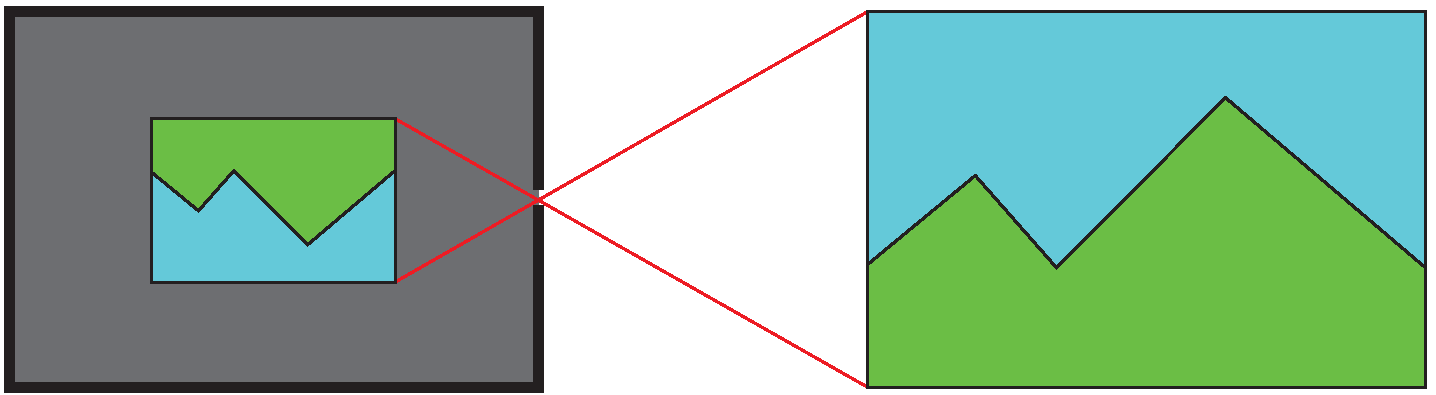
\includegraphics[width=\textwidth]{images/camera oscura.pdf}
\end{figure}

Con questa configurazione l'immagine risulta riflessa rispetto al mondo esterno.
Utilizziamo quindi un ulteriore astrazione, in cui poniamo il sensore al di fuori della camera, mantenendo però la condizione in cui la luce deve passare per l'apertura puntiforme per essere catturato nell'immagine (figura \ref{fig:camera model}).
È facilmente verificabile che l'immagine così ottenuta sia uguale all'immagine precedente ma riflessa, e quindi sia coerente con la realtà.
\begin{figure}
    \caption{Sensore esterno alla camera}
    \label{fig:camera model}
    \centering
    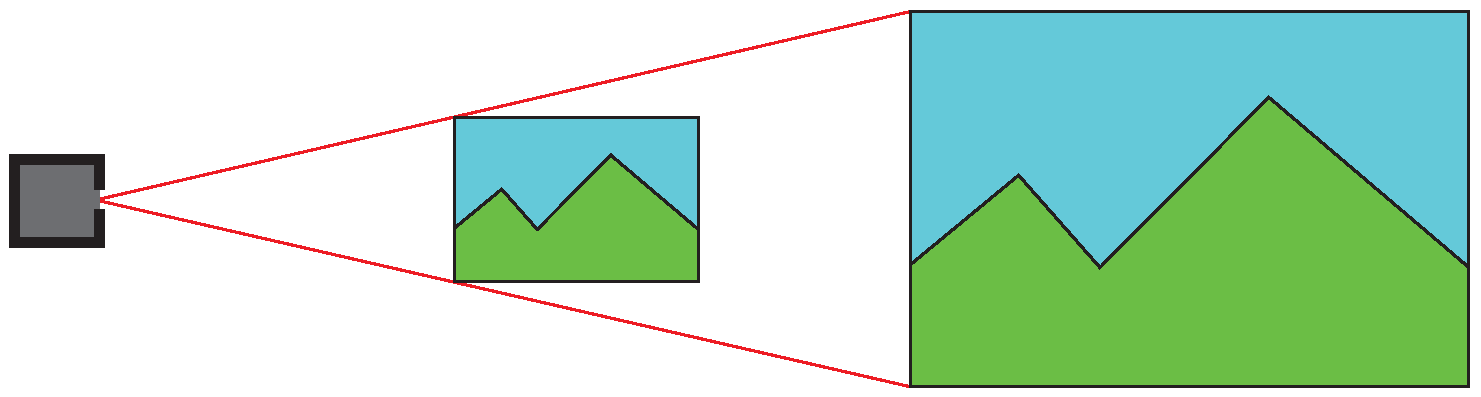
\includegraphics[width=\textwidth]{images/camera astratta.pdf}
\end{figure}

Ciò a cui siamo interessati non è però generare l'immagine, ma conoscere la configurazione dello spazio reale con cui l'immagine è stata generata.
Dato che l'immagine è generata da raggi di luce che si muovono in linea retta possiamo affermare che ad ogni punto $P'$ dell'immagine corrisponde un punto $P$ nello spazio reale e che questo punto si trova sulla linea che passa per la camera e $P'$.
Questo non è abbastanza per individuare $P$, in quanto una linea contiene infiniti punti.
Possiamo risolvere questo problema conoscendo il contesto che stiamo provando a correggere.
Dato che questo contesto è il contesto stradale, possiamo supporre che le entità a cui siamo interessati siano poggiate sulla strada, che approssimiamo con un piano bidimensionale.
Il punto $P$ è quindi contenuto sia nel raggio di luce che nel piano stradale.
Assegnamo delle coordinate ai vari elementi per calcolare la trasformazione (figura \ref{fig:camera coords}).
\begin{figure}
    \caption{Modello con coordinate}
    \label{fig:camera coords}
    \centering
    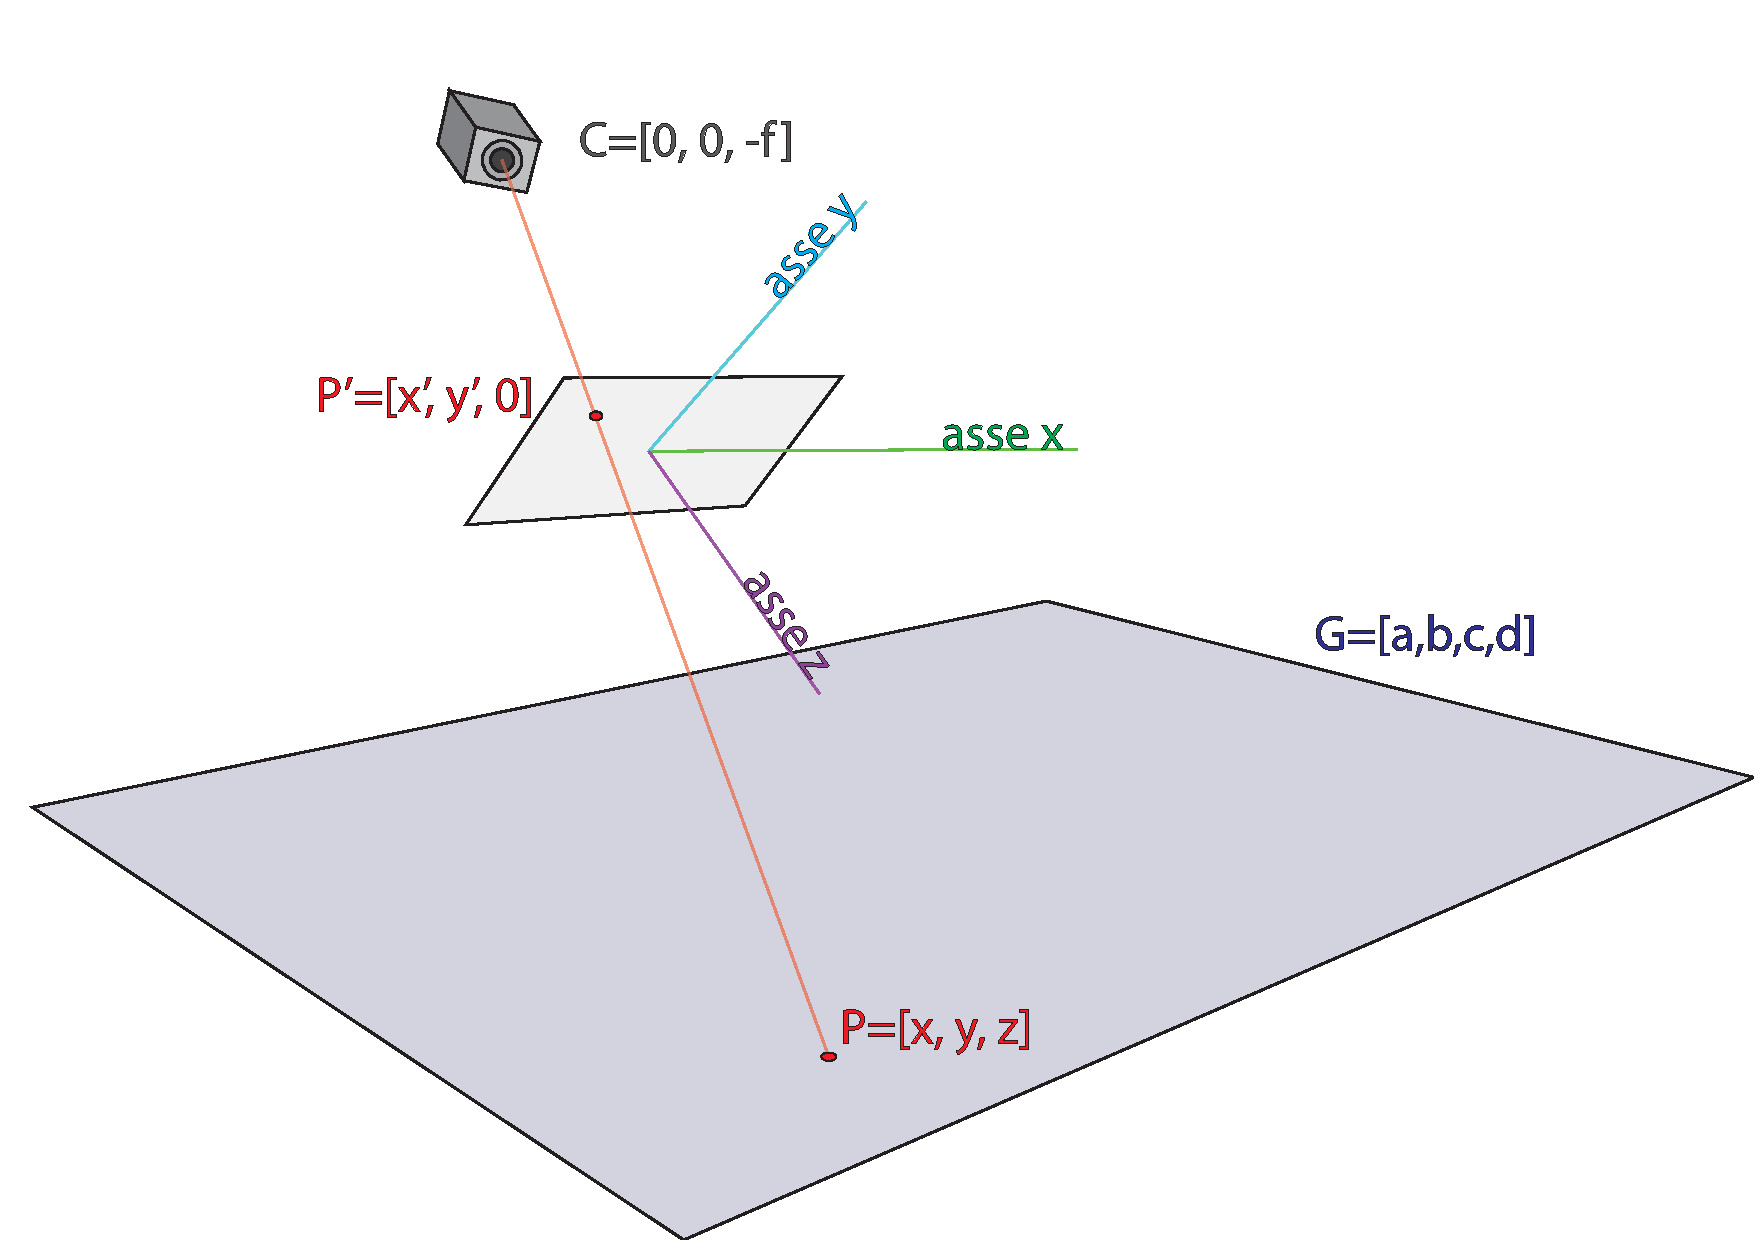
\includegraphics[width=\textwidth]{images/camera coords.pdf}
\end{figure}

Possiamo ricavare il punto $P$ trovando l'intersezione tra il piano $G$ e la linea $\overline{CP'}$.
In $R^3$ una linea è identificata da un sistema di 2 equazioni.
Il punto $P$ è quindi definito dal sistema di 3 equazioni in \ref{eq:system}.
\begin{equation}
    \label{eq:system}
    P = 
    \left\{
    \begin{aligned}
         & ax + bx + cz + d = 0                       \\
         & \frac{1}{x'}x - \frac{1}{y'}y + 0z + 0 = 0 \\
         & 0x -  \frac{1}{y'}y + \frac{1}{f}z + 1 = 0 \\
    \end{aligned}
    \right.
\end{equation}

Risolvendo il sistema in \ref{eq:system} troviamo le equazioni in \ref{eq:cartesian}.
\begin{equation}
    \label{eq:cartesian}
    \begin{aligned}
         & x = \left( \frac{cf - d}{ax' + by' + cf} \right) x'    \\
         & y = \left( \frac{cf - d}{ax' + by' + cf} \right) y'    \\
         & z = \left( \frac{cf - d}{ax' + by' + cf} - 1 \right) f \\
    \end{aligned}
\end{equation}
Le equazioni così trovate non sono lineari.
Possiamo però definire una nuova coordinata $\lambda$ e trasformare le equazioni in \ref{eq:cartesian} nelle equazioni in \ref{eq:homogeneous}.
\begin{equation}
    \label{eq:homogeneous}
    \begin{aligned}
        \lambda x & = (cf - d) x'       \\
        \lambda y & = (cf - d) y'       \\
        \lambda z & = -fax' - fby' - fd \\
        \lambda   & = ax' + by' + cf    \\
    \end{aligned}
\end{equation}

Le coordinate $[\lambda x, \lambda y, \lambda z, \lambda]^T$ sono chiamate \emph{coordinate proiettive omogenee}.
La forma normale $N$ di un vettore $V$ definito in \emph{coordinate proiettive omogenee} si ottiene attraverso la formula $N = \displaystyle\frac{V}{\lambda_V}$.
$N$ è quindi della forma $N = [x, y, z, 1]^T$.
È perciò semplice la conversione da \emph{coordinate cartesiane} a \emph{coordinate proiettive} e viceversa.
Possiamo quindi definire le equazioni trovate come trasformazione lineare in coordinate proiettive.
La matrice relativa a questa trasformazione è in \ref{eq:projmat}.
\begin{equation}
    \label{eq:projmat}
    J_{(f, [a, b, c, d])} =
    \begin{bmatrix}
        cf - d & 0      & 0   \\
        0      & cf - d & 0   \\
        -fa    & -fb    & -fd \\
        a      & b      & cf  \\
    \end{bmatrix}
\end{equation}
Questo sistema di coordinate è lo stesso utilizzato per applicare le classiche trasformazioni lineari di traslazione, rotazione, scala e shear.
Tutte queste trasformazioni rimangono quindi applicabili anche dopo il cambio di coordinate e possono essere combinate con la trasformazione di proiezione $J$ trovata.

Riassumiamo i passaggi da compiere in modo da comporre la trasformazione $M$ completa:
\begin{enumerate}
    \item Cambiare coordinate da $R^2$ omogeneo in $R^3$ omogeneo, settando $z=0$.
    \item Scalare l'immagine, rendendo $h = 1, w = w/h$.
    \item Riflettere l'asse Y dell'immagine, in modo che incrementi muovendosi verso l'alto.
    \item Traslare l'origine dell'immagine al centro di questa.
    \item Proiettare l'immagine sul piano $G$, calcolando e applicando $J$.
    \item Applicare l'inversa della trasformazione dell'immagine, così da avere $z=0$ per tutti i punti ottenuti.
    \item Rimuovere la coordinata $z$, così da tornare in $R^2$ omogeneo.
\end{enumerate}
Per calcolare il piano $G$, necessario per calcolare $J_{(f, G)}$, si deve:
\begin{enumerate}
    \item Applicare al piano $[0, 0, 1, 0]$, che è il piano in cui $z=0$, l'inversa della rotazione dell'immagine.
    \item Calcolare l'origine del piano $O$, applicando l'inversa della trasformazione dell'immagine al punto $[0, 0, 0, 1]$.
    \item Applicare al piano la ``traslazione per piani'' che porta l'origine nel punto calcolato in precedenza. Questa ``traslazione per piani'' è uguale alla trasposta dell'inversa della traslazione per punti.
\end{enumerate}
Quindi abbiamo, indicando come $I$ la trasformazione completa dell'immagine, $I_R, I_T$ rispettivamente rotazione e traslazione dell'immagine, $T_{(x, y, z)}$ la traslazione che porta $[0, 0, 0, 1]$ in $[x, y, z, 1]$, $S_{(x, y, z)}$ la scala che porta $[1, 1, 1, 1]$ in $[x, y, z, 1]$:
\begin{equation}
    \begin{aligned}
        O & = I^{-1} \cdot [0, 0, 0, 1]                       \\
        G & = T_{(O)}^{-1T} \cdot I_R^{-1} \cdot [0, 0, 1, 0] \\
        M & =
        \begin{bsmallmatrix}
            1 & 0 & 0 & 0 \\
            0 & 1 & 0 & 0 \\
            0 & 0 & 0 & 1 \\
        \end{bsmallmatrix}
        \cdot I^{-1} \cdot J_{(f, G)} \cdot T_{(0.5, w/2h)} \cdot S_{(1/h, -1/h, 1)} \cdot
        \begin{bsmallmatrix}
            1 & 0 & 0 \\
            0 & 1 & 0 \\
            0 & 0 & 0 \\
            0 & 0 & 1 \\
        \end{bsmallmatrix}                                   \\
    \end{aligned}
\end{equation}
La matrice $M$ trovata è una matrice $3x3$.
È perciò una matrice omografica in $R^2$ omogeneo.
Il punto $P = M \cdot P'$ deve perciò essere normalizzato e convertito in coordinate cartesiane prima di essere utilizzato dal resto del sistema.
